\documentclass[class=article, crop=false]{standalone}
\usepackage{my_preamble}
\begin{document}
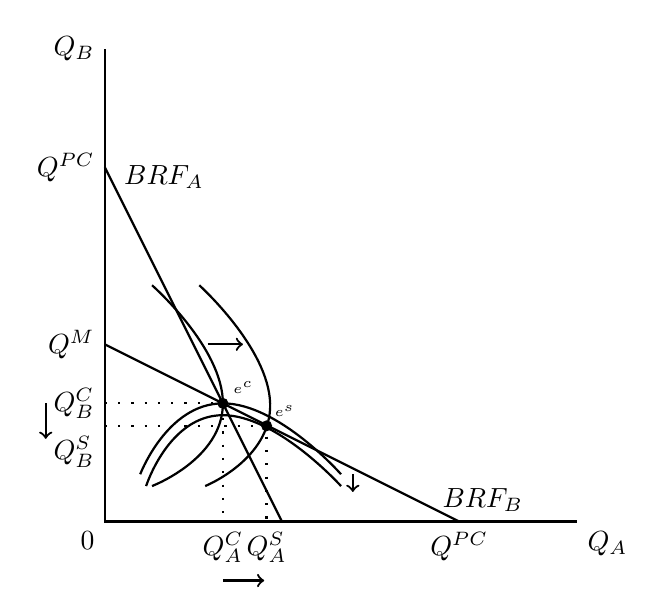
\begin{tikzpicture}[thick,font=\sffamily,scale=1.5]
	%axis
	 \draw (0,4) node[left]{$Q_{B}$} -- (0,0) node[below left] {$0$} -- (4,0) node[below right]{$Q_{A}$};
	  
	 %BRFs
	\draw[] (0,3) -- (1.5,0); %BRF A
	\draw[] (0,1.5) -- (3,0); %BRF B

	%Iso-profits
	\draw[] plot [smooth, tension=1] coordinates {(0.3,0.4) (1,1) (2,0.4)}; %A's iso-profit 1
	\draw[] plot [smooth, tension=1] coordinates {(0.35,0.3) (1,0.9) (2,0.3)}; %A's iso-profit 2
	\draw[] plot [smooth, tension=1] coordinates {(0.4,0.3) (1,1) (0.4,2)}; %B's iso-profit 1
	\draw[] plot [smooth, tension=1] coordinates {(0.85,0.3) (1.4,1) (0.8,2)}; %B's iso-profit 2
	
	%labels
	\node[below] at (0.5,3.1) {$BRF_{A}$}; %BRF A label
	\node[above] at (3.2,0) {$BRF_{B}$}; %BRF B label
	%\node[below] at (1.5,0) {$Q^{M}_A$}; %A's monopoly quantity
	\node[left] at (0,1.5) {$Q^{M}$}; %B's monopoly quantity
	\node[below] at (3,0) {$Q^{PC}$}; %PC quantity - A's???
	\node[left] at (0,3) {$Q^{PC}$}; %PC quantity
	
	%equilibria labels
	\node[style={fill=black,circle,inner sep=0pt,minimum size=4pt}] at (1,1) { };
	\node[above right]at (1,1) {\tiny{$e^{c}$}};
	\node[style={fill=black,circle,inner sep=0pt,minimum size=4pt}] at (1.37,0.81) { };
	\node[above right]at (1.35,0.8) {\tiny{$e^{s}$}};
	
	%dotted lines	
	\draw[loosely dotted] (0,1) node[left]{$Q^{C}_B$} -| node[pos=0.25,below=3mm] {}
	  (1,0) node[below]{$Q^{C}_A$}; %cournot dotted lines
	\draw[loosely dotted] (0,0.81) node[below left]{$Q^{S}_B$} -| node[pos=0.25,below=3mm] {}
	  (1.37,0) node[below]{$Q^{S}_A$}; %stackelberg dotted lines
	
	%arrows
	\draw [->] (1,-0.5) -- (1.35,-0.5); %x arrow
	\draw [->] (-0.5,1) -- (-0.5,0.7); %y arrow
	\draw [->] (0.87,1.5) -- (1.17,1.5); %A's arrow
	\draw [->] (2.1,0.4) -- (2.1,0.25); %B's arrow
\end{tikzpicture}
\end{document}